\documentclass{ltjsbook}
\usepackage{docmute} 
\usepackage{../../myStyle} 

\begin{document}
\chapter{行列計算の基礎}
\label{L01_LinearAlgebra}
\section{線形代数とは何なのか}
\subsection{便利な表現方法としての線形代数}
今から線形代数を学んでいくわけですが，はじめに「線形代数とは何で，なぜ(心理学者が)学ぶのか」について説明しておきましょう。というのも，線形代数の数学書は世の中にたくさんあるわけですが，理由についてはせいぜい，多変量解析をするにあたって行列は必須だ，と書いてあるぐらいだからです。まるで野球の楽しさを知るためにルールブックを読め，と言っているようなものですから，文系の心理学者にとって，これでは面白みが見えてこないでしょう。

このコースの受講生は，心理統計はひととおり学んでいる，統計ソフトウェアは使ったことがあるというぐらいの基礎知識を持っている人を前提にしていますから，データがスプレッドシートに入っているシーンを想像してください，といえばイメージしてもらえますでしょうか。
心理学ではデータを取って，一行に一人分のデータを入れていく，変数は列方向に並べていく，というルールが基本です\footnote{これはワイド型，あるいは横長型のデータ入力の方法です。これとは別に，ロング型・縦長型のデータという入力方法もあります。またデータの入力規則としては，統計ソフトウェアが計算しやすいデータの持ち方として\citet{Hadley2014}が提唱した\keyterm{整然データ}{せいぜんでーた}{Tidy Data}という考え方も知っておいて損はありません。}。ここまでの説明ですでに「行」「列」という言葉を使ってしまいましたが，このようにデータは\keyterm{行列}{ぎょうれつ}{matrix}で全体を表現できます。

心理学者はこのデータ行列から，意味のある知見を取り出そうとして，平均や分散の計算をしたり，相関係数や回帰係数の計算をしたりするわけですから，このデータ行列にすべての情報が詰まっているはずです。表計算ソフトでは，列毎，行毎の統計量を計算できますが，それはデータの一部分に限定した使い方ですね。もちろん相関係数など複数の行をつかって計算することはありますが，数十の変数列を一気に操作するには表計算ソフトではなく，統計パッケージが必要ですね。その違いは，行列の計算をするか，線形代数の操作をするかどうかだと言ってもいいでしょう\footnote{ええ，もちろんわかっていますよ，分析ツールやVBAをつかえばエクセルでお行列の計算ができるじゃないか，というご意見があるのは。}。つまり，複数の変数を同時に使う分析，たとえば重回帰分析や因子分析などがそうですが，そこには線形代数というツールが裏で働いているわけです。

つまり線形代数は，複数の数字のセットを扱うための計算方法だということです。文字や記号をつかった数学や方程式，関数といえば，$x,y$などアルファベット2,3種類が精々だったかもしれませんが，YG性格検査などは120項目あるわけですから120文字必要で，そうなるともっと一般化した表現，まとめて扱うツールが必要ですね。それが線形代数なのです。

線形代数は新しい表現方法だ，と思っていただければ良いかと思います。変数をまとめて，リストにして扱うわけですから，今までとは違う書き方をし，違う計算ルールが必要になります。利点は「まとめて扱う」ことを最初から目的にしていますから，変数3つだろうが4つだろうが，120個あっても同じように表現できるようになっているところです。つまり，データのサイズについて一般化した話ができるということです！

線形代数の表現に慣れると，変数のリストのまま，スプレッドシート全体像をイメージしたまま，加減乗除の加工ができるようになります。非常にサイズが大きくなることもあり得ますし，なにより新しい表現方法，計算方法に慣れないといけません。線形代数が難しいのでは，と身構えする人もいるかもしれませんが，ここでの難しさは，正確に言うと「単純な操作だがたくさん反復しないといけないので，途中でミスが生じやすい」ことによる成功体験の得難さ，つまり「煩雑さ」が原因です。複素関数や測度論などのような\underline{「抽象的すぎて理解が困難だ」というタイプの難しさではない}のです。逆に言うと面倒だけどシンプルなので，計算のパターンが身につきさえすれば，あとは反復計算が得意な計算機に任せてしまって構いません。自転車に乗る練習をするように，最初は根気が必要ですが，後は雰囲気で使うことができる便利なものだと思ってください。
\subsection{線形代数を会得すると見えてくる世界}
線形代数は数字のリストを扱う，という話をしました。今まで習った数字・変数のリストといえば，連立方程式がおもいつくかもしれません。まさに，線形代数は連立方程式を簡単に扱うための表現方法という側面もあります。

もうひとつ，複数の数字をまとめて扱うのは座標などの空間の話です。$(x,y)=(2,3)$のように座標は2つの数字が組になって，ある位置を表すのでした。3次元空間でしたら，$(x,y,z)$のように3つ組で表現します。線形代数はこうした空間的表現にも，新しい理解やイメージを与えてくれます。連立方程式の解を関数の交点で求めたように，式を空間で表現することもできるわけです。

さて私たちは120項目からなる1000人分のデータセットを分析する，なんてことをしたりするわけですが，これも120次元，1000次元の空間として表現してもいいですよね。もちろん可視化するのは3次元が限界ですが，数学の世界の中では$n$次元空間と一般化して考えることができます。このように，データをベクトルとして考え，それがなんらかの空間を持っている，という想像することが可能です。ではその空間において，回帰分析はどういう意味があるのでしょう? 主成分分析や因子分析はどういうことをしているのか，空間のメタファーで考えるとどうでしょう? このように，多変量のデータ分析の空間的なイメージ，幾何学的な想像をはたらかせることで，分析モデルの理解が一層進むことが期待されます。たとえば因子分析においては因子数の決定をするときにスクリープロットを見るという方法がありますが，あれは何をみていて，どういう意味があるのかは，線形代数の空間的イメージを経由すると直感的に理解できます。あるいはまた，重回帰分析において多重共線性があると良くないという話がありますが，どうしてダメなのかということについても図式的に理解できます。

データセットを数字の羅列と見て計算することもできるし，データセットを空間にあるベクトルと考えることもできる，この両方の視点を提供してくれるのが線形代数です\footnote{一般にデータサイエンティストやコンピュータサイエンティストは，数字の羅列として考えることが多いでしょう。これに対して，物理学では空間における力の表現としてのベクトル，つまり始点・方向・大きさがセットになったものの表現として線形代数を扱います。数学ではこの両方の視点を行き来できるような，一般的な操作を考えています。数字のリストと空間の表現のいいとこ取りをテーマに作られた，Essence of linear algebraというYoutube動画(\url{https://bit.ly/3abXiFz})は一見の価値があります。}
何事についても，多角的な理解をすること，さまざまな言葉で表現できることが「わかっている」ということの本質だと思います。皆さんも数字のリスト，それの作る空間を同時に想像しながら，自らの分析モデルの理解への一助としてください。

\section{行列の定義}
\subsection{行列とベクトル}
行列やベクトルは，複数の数字をひとまとめにして扱うためのものです。まずはその基本的な形からみていきます。

\subsubsection{ベクトル}
複数の数字を一行，あるいは一列にまとめて表現したものを，\keyterm{行ベクトル}{ぎょうべくとる}{row vector},\keyterm{列ベクトル}{れつべくとる}{column vector}といいます。

行ベクトルは次のように表します。
\begin{equation*}
    \bm{a}=
    \begin{pmatrix}
        a_1 & a_2 & \cdots & a_m
    \end{pmatrix}
\end{equation*}

列ベクトルは次のように表します。
\begin{equation*}
    \bm{b}=
    \begin{pmatrix}
        b_1 \\ b_2\\ \vdots \\ b_m
    \end{pmatrix}
\end{equation*}

具体的には，$a_1$とか$b_2$のところには数字が入っています。つまり次のような形です。
\begin{equation*}
    \bm{a}=
    \begin{pmatrix}
        1 & 3 & 5
    \end{pmatrix},
    \bm{b}=
    \begin{pmatrix}
        2 \\ 4\\ 6\\ 12 \\ 8
    \end{pmatrix}
\end{equation*}

ここで今回の$\bm{a}$は3つの要素が入っていますので，サイズは3，同じく$\bm{b}$はサイズが5のベクトルです。行列の言い方に合わせて$1 \times 3$の(行)ベクトル，$5 \times 1$の(列)ベクトル，とみることもできますし，それぞれ3次元，5次元空間のベクトルと考えても構いません。
ちなみに行は$\to$の方向，列は$\downarrow$の方向です。行という漢字の四画目，列という漢字の最後の一画が方向を表している，と覚えるといいかもしれません\footnote{行の最後の一画，列の最初の一画と逆に覚えないように!}。ちなみに英語で行はRow，列はColumnで，Rの下を伸ばしたり，Lが縦長なのでそれを意識したりして，方向を覚えるといいかもしれません(図\ref{fig::01_01})。

\begin{figure}[h]
    \begin{center}
        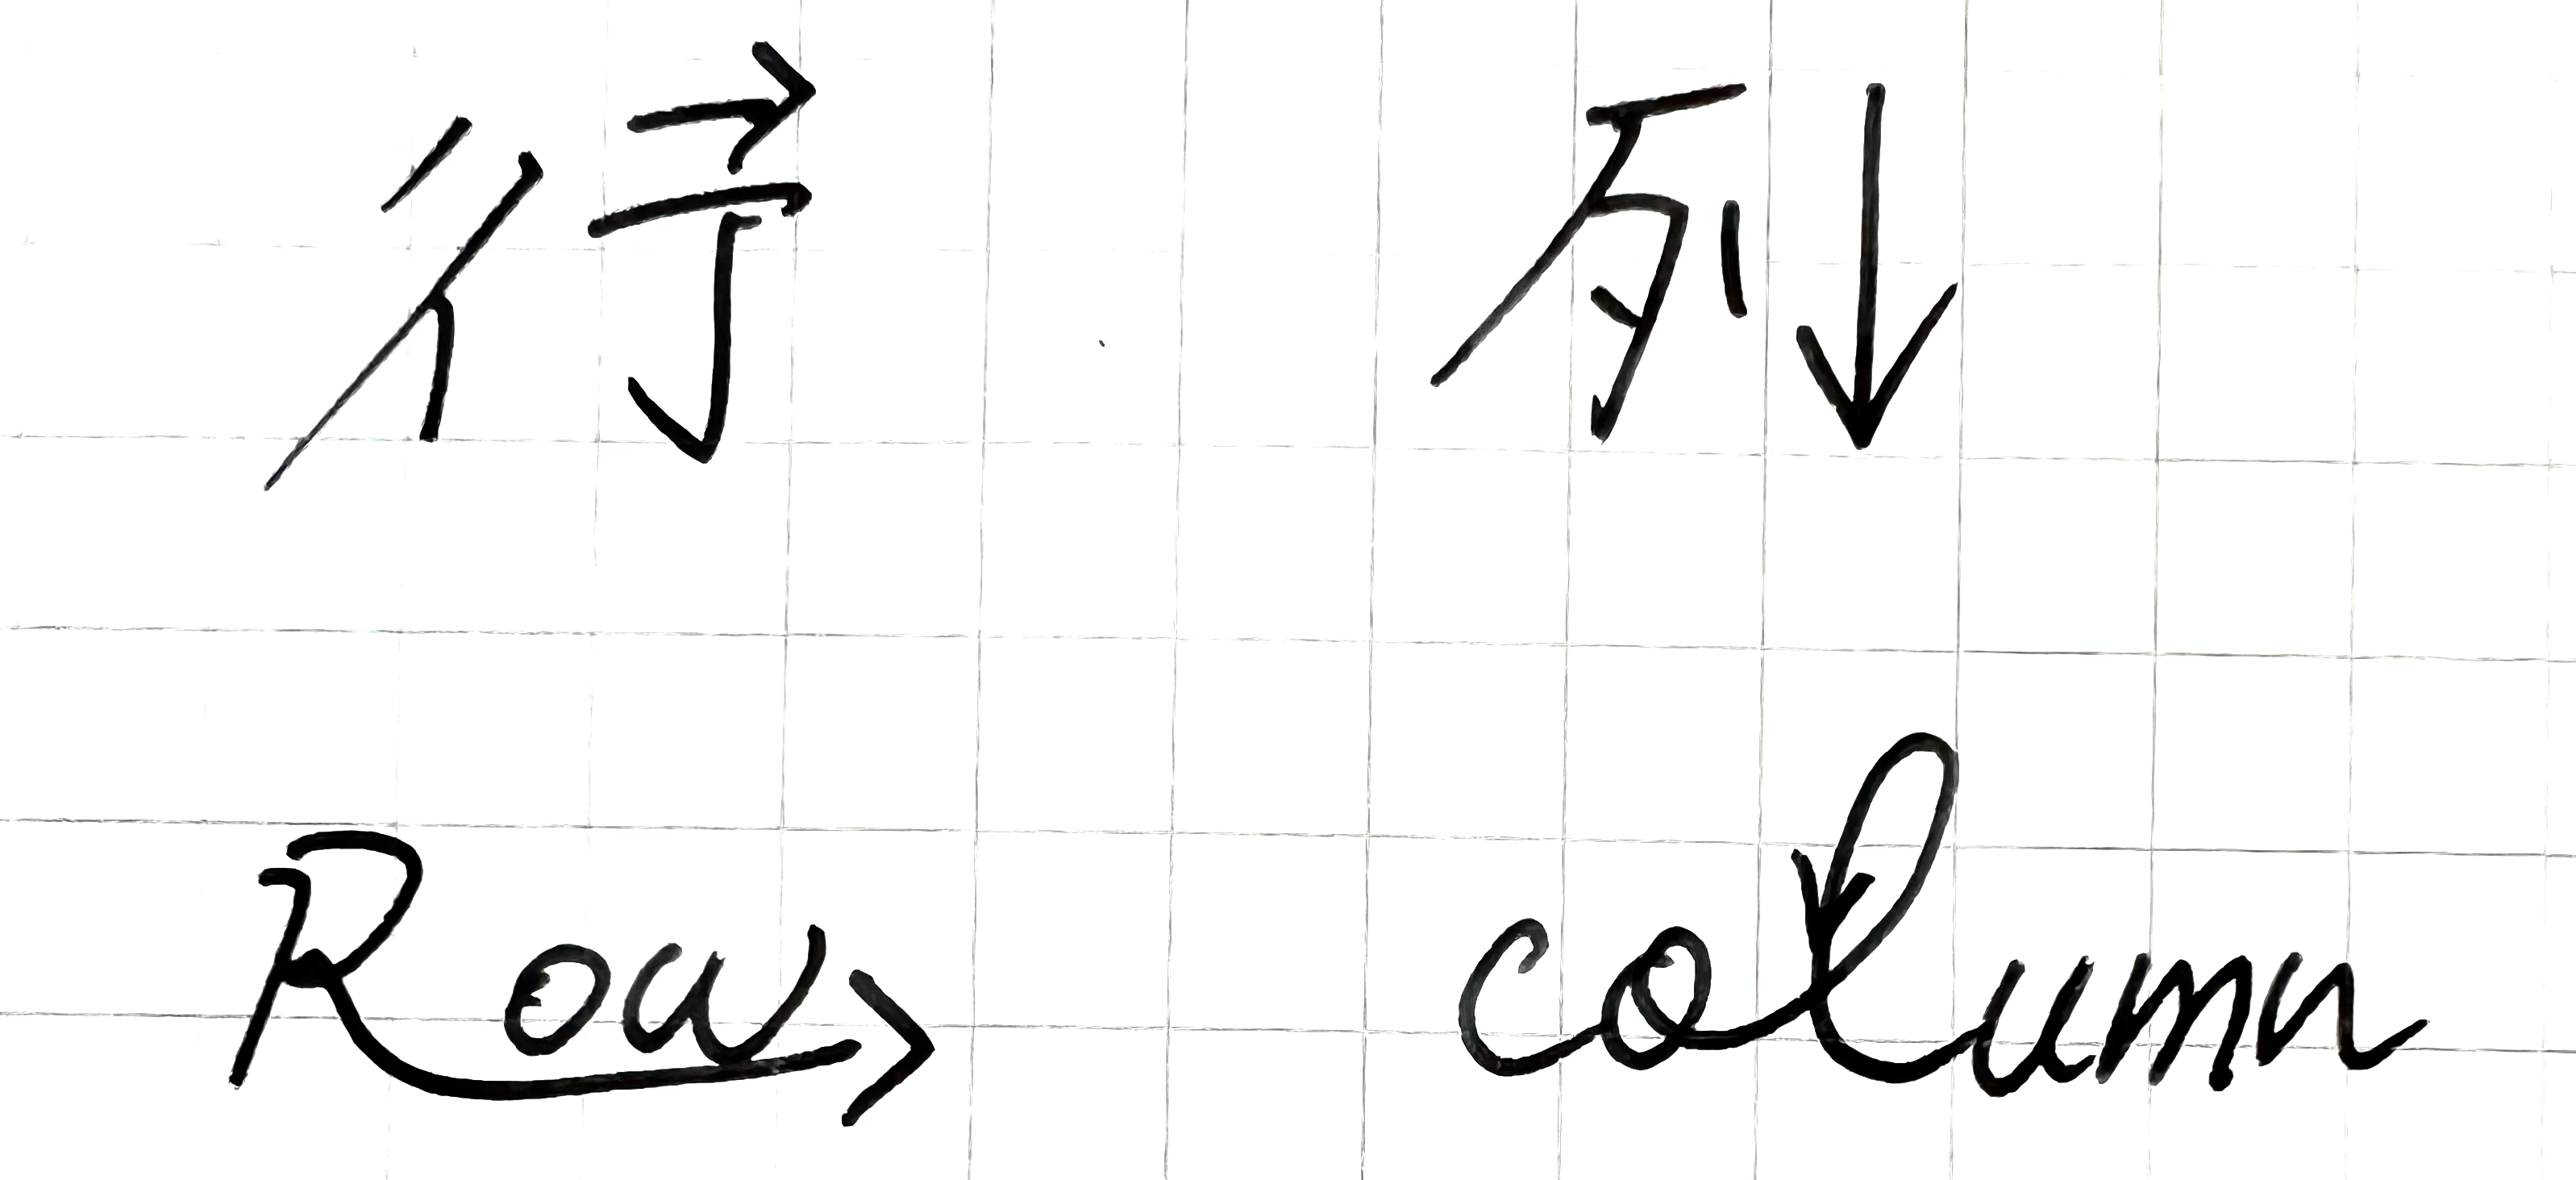
\includegraphics[width=0.5\linewidth,keepaspectratio]{../images/LA01/RowColumn.png}
        \caption{行と列，その覚え方}
        \label{fig::01_01}
    \end{center}
\end{figure}

また，ベクトルやこの後出てくる行列を表すアルファベットは，$a$や$B$のようにただのアルファベットではなく，$\bm{a}$，$\bm{B}$のように\ruby{太字体}{ボールド}で表します。字が太くなっているときはベクトルや行列，すなわち複数の数字から構成されたものだな，と思って見るようにしてください。ちなみに手書きでノートなどに書くときは，どこかの一画を二重線にするなどして表現することが多いです。

閑話休題。このベクトルの中の数字は，とくに関係があるわけではありません。前に入っている数字がえらいとか，横にある方が重要だ，といったことはなく，ただただ数字をまとめて扱っているだけです。本来別々の数字なのです。たとえば身長と体重という2つの変数があったとき，ある人のデータを$ \begin{pmatrix} 170 \\ 60 \end{pmatrix} $と表すことができます。全然別の種類の，別の単位の数字ですね。ただし，一行目の要素に身長，二行目の要素に体重を入れるという規則にしたのであれば，別の人のデータも$\begin{pmatrix} 150 \\ 45 \end{pmatrix}$のように表さなければなりません。ここで要素の順番を入れ替えることはできないのです。

さて，行数も列数も1であるものつまり行列でない数字は，とくに\keyterm{スカラー}{すからー}{scalar}と呼びます。今までは$1+2=3$といった計算をしていましたが，この$1,2,3$はすべてスカラーだといえるわけです。
「スカラー」という用語は線形代数の専門用語として定着していますが，\ruby{Scale}{スケール}を扱うもの，という意味があるので「スケイラー」と発音した方がわかりやすいかもしれません。この後，スカラーとベクトル・行列の積の話をしますが，定数倍のように大きさを変えるという操作をします。空間的な表現のイメージとつなげることの利点が，そんなところにも現れてくるのですね。

\subsubsection{行列}
\keyterm{行列}{ぎょうれつ}{matrix}とは数を長方形に並べたものです。行列として並べられた数を成分といい，成分の横の並びを行，縦の並びを列と呼びます。

\begin{equation*}
    \bm{A}=
    \begin{pmatrix}
        a_{11} & a_{12} & \cdots & a_{1j} & \cdots & a_{1m} \\
        a_{21} & \ddots &        & \vdots &        & a_{2m} \\
        \vdots &        & \ddots & \vdots &        & \vdots \\
        a_{i1} & \cdots & \cdots & a_{ij} &        & \vdots \\
        \vdots &        &        &        & \ddots & \vdots \\
        a_{n1} & a_{n2} & \cdots & \cdots & \cdots & a_{nm} \\
    \end{pmatrix}
\end{equation*}


この例は，$n$行$m$列の行列を表しています。この行列の成分を表す文字は，一般に$a_{ij}$のように，はじめの添え字で行番号，次の添え字で列番号を表します。行列の大きさは行数と列数とによって，$n \times m$のように表現します。
表計算ソフトなどで見る，シートの中に入っているデータセットを考えると，行が個人・ケース・Observationsを表していて，列が変数を表しているのが一般的ですね。行列を考えるときは$n$が数百人ぐらい，$m$が数十ぐらいのサイズでイメージすると良いと思います。調査系のデータであれば，$n$が3,4桁ぐらい，$m$が2桁台なのが一般的ではないかと思います。$n>m$の縦に長い長方形を頭に思い描いてみてください。行列では，このサイズ感(サイズのイメージ)が特に重要です。

\paragraph{正方行列}
一方，$n$と$m$が同じ，つまり行数と列数が同じであれば正方形になりますから，これをとくに\keyterm{正方行列}{せいほうぎょうれつ}{Square Matrix}といいます。正方行列の例を次にあげておきます。


\begin{equation*}
    \bm{A} =
    \begin{pmatrix}
        1 & 2 & 3 \\
        4 & 5 & 6 \\
        7 & 8 & 9
    \end{pmatrix}
\end{equation*}

\paragraph{対称行列}

正方行列の中でも，$i$行$j$列目の値が$j$行$i$列目の値と同じである行列($a_{ij}=a_{ji}$)のことを\keyterm{対称行列}{たいしょうぎょうれつ}{Symmetric Matrix}といいます。

\begin{equation*}
    \bm{A} =
    \begin{pmatrix}
        1 & 2 & 3 \\
        2 & 5 & 6 \\
        3 & 6 & 9
    \end{pmatrix}
\end{equation*}

この(正方)対称行列の形は，データ解析の計算途中でよくでてきます。たとえば3つの変数$x_1,x_2,x_3$について，その相関係数を考えたいとしましょう。相関係数は2つの数字の組み合わせですから，$x_1$と$x_2$，$x_1$と$x_3$，$x_2$と$x_3$について計算でき，それぞれ$r_{12},r_{13},r_{23}$と表したとします。$i$と$j$の相関係数$r_{ij}$は，$j$と$i$の相関係数と同じ($r_{ij}=r_{ji}$)であり，また$r_{jj}=1.0$なのは定義から明らかです。これを行列で表すと次のようになります。

\begin{equation*}
    \bm{R} =
    \begin{pmatrix}
        1      & r_{12} & r_{13} \\
        r_{21} & 1      & r_{23} \\
        r_{31} & r_{32} & 1
    \end{pmatrix}=
    \begin{pmatrix}
        1      & r_{12} & r_{13} \\
        r_{12} & 1      & r_{23} \\
        r_{13} & r_{23} & 1
    \end{pmatrix}
\end{equation*}

$r_{ij}=r_{ji}$ですから，対称行列になっています。この行列をとくに\keyterm{相関行列}{そうかんぎょうれつ}{Correlation Matrix}といいます。また相関係数は標準化された共分散でもありました。標準化するまえの相関行列は，\keyterm{分散共分散行列}{ぶんさんきょうぶんさんぎょうれつ}{Covariance Matrix}と言います。その名前の通り，自分自身との共分散が分散になるわけですから，右上から右下にかけての対角線上にある要素(これをとくに\keyterm{対角}{たいかく}{diagonal}要素といいます)が分散であり，それ以外が共分散になっている行列です。

\begin{equation*}
    \bm{V} =
    \begin{pmatrix}
        s_1^2  & s_{12} & s_{13} \\
        s_{21} & s_2^2  & s_{23} \\
        s_{31} & s_{32} & s_3^2
    \end{pmatrix}
\end{equation*}

\paragraph{対角行列と単位行列}
また，正方行列の中でもとくに対角要素にのみ値があって，それ以外はすべて$0$になっている行列のことを\keyterm{対角行列}{たいかくぎょうれつ}{diagonal matrix}といいます。
\begin{equation*}
    \begin{pmatrix}
        a_{11}                                                 \\
         & a_{22}          &        & \text{\huge{0}}          \\
         &                 & \ddots                            \\
         & \text{\huge{0}} &        & \ddots                   \\
         &                 &        &                 & a_{nn}
    \end{pmatrix}
    =
    \begin{pmatrix}
        a_{11}                               \\
         & a_{22} &        & \bm{O}          \\
         &        & \ddots                   \\
         & \bm{O} &        & \ddots          \\
         &        &        &        & a_{nn}
    \end{pmatrix}
\end{equation*}

ここで表されているように，対角要素以外は全てゼロですから，ゼロを大きく太字で書いたり，オーを使って$\bm{O}$としてここは空っぽだよ，ということを意味することがあります。

また対角行列の中でもとくに，対角項が1になっているものは\keyterm{単位行列}{たんいぎょうれつ}{identity matrix}と呼びます。単位行列は$\bm{I}$とか
$\bm{E}$で表されます。


\begin{equation*}
    \bm{I} =
    \begin{pmatrix}
        1      & 0      & \cdots & 0      \\
        0      & 1      & \cdots & 0      \\
        \vdots & \vdots & \ddots & \vdots \\
        0      & 0      & \cdots & 1      \\
    \end{pmatrix} =
    \begin{pmatrix}
        1                                                 \\
         & 1               &        & \text{\huge{0}}     \\
         &                 & \ddots                       \\
         & \text{\huge{0}} &        & \ddots              \\
         &                 &        &                 & 1
    \end{pmatrix}
\end{equation*}


これは後ほど，掛け算をするときに「かけても変わらない状態」を表すために用いられます。$\bm{I}_n$のように表すことで，サイズ$n \times n$の単位行列であることを意味することもあります。単位行列は計算過程でよく出てくる行列で，特に式中でサイズを明示しないこともありますが，計算過程を考えるとそのサイズはじめいであるので，「計算できるような適当なサイズ」である，と思っていただいてもいいかもしれません。

\section{行列の四則演算}
行列の四則演算は，通常のスカラーのそれとは異なります。改めて，行列としての加減乗除を定義するのだと思ってください。
\subsection{ベクトルの計算}
\paragraph{ベクトルの足し算・引き算}
\paragraph{ベクトルとスカラーの積}
\paragraph{ベクトルとベクトルの積}

\subsection{行列の計算}
\paragraph{行列のの足し算・引き算}
\paragraph{行列とスカラーの積}
\paragraph{行列とベクトルの積}
\paragraph{行列と行列の積}





\paragraph{加法・減法}
まずは行列の足し算(加法)，引き算(減法)から説明します\footnote{ベクトルは行列の中でも，行数あるいは列数が1のものですので，これで一般的に表現します。} 。これはそれぞれ対応する位置にある成分を加え合わせる(減じる)ことで表されます。

\begin{equation*}
    \bm{A}+\bm{B} =
    \begin{pmatrix}
        a_{11}+b_{11} & a_{12}+b_{12} & \cdots & a_{1m}+b_{1m} \\
        a_{21}+b_{21} & a_{22}+b_{22} & \cdots & a_{2m}+b_{2m} \\
        \vdots        & \vdots        & \ddots & \vdots        \\
        a_{n1}+b_{n1} & a_{n2}+b_{n2} & \cdots & a_{nm}+b_{nm} \\
    \end{pmatrix}
\end{equation*}

数値例をみておきましょう。
\begin{equation*}
    \begin{pmatrix}
        1 & 2 \\
        3 & 4
    \end{pmatrix}
    +
    \begin{pmatrix}
        5 & 6 \\
        7 & 8
    \end{pmatrix}
    =
    \begin{pmatrix}
        1+5 & 2+6 \\
        3+7 & 4+8
    \end{pmatrix}
    =
    \begin{pmatrix}
        6  & 8  \\
        10 & 12
    \end{pmatrix}
\end{equation*}

これからわかるように，行列の加法，減法は大きさの等しい行列でないと成り立ちません。サイズが違うものを足そうとすると，演算できない箇所が出てしまうのです。このように行列では，\underline{「計算できない」という状態になることが}ありえます。行列のサイズに注意が必要，ということがお分かりいただけるかと思います。


\paragraph{乗法}
続いて掛け算です。まずスカラーと行列の積を見てみましょう\footnote{指揮中にでてくる$\lambda$はギリシア文字でラムダといいます。小文字が$\lambda$，大文字では$\Lambda$と書きます。}。

\begin{equation*}
    \lambda \bm{A} = \bm{A} \lambda =
    \begin{pmatrix}
        \lambda a_{11} & \lambda a_{12} & \cdots & \lambda a_{1m} \\
        \lambda a_{21} & \lambda a_{22} & \cdots & \lambda a_{2m} \\
        \vdots         & \vdots         & \ddots & \vdots         \\
        \lambda a_{n1} & \lambda a_{n2} & \cdots & \lambda a_{nm} \\
    \end{pmatrix}
\end{equation*}


実際の計算は，各成分をスカラー倍すればよいだけですので，比較的簡単ですね。

\begin{equation*}
    2 \times
    \begin{pmatrix}
        1 & 2 \\
        3 & 4
    \end{pmatrix}
    =
    \begin{pmatrix}
        2 \times 1 & 2 \times 2 \\
        2 \times 3 & 2 \times 4
    \end{pmatrix}
    =
    \begin{pmatrix}
        2 & 4 \\
        6 & 8
    \end{pmatrix}
\end{equation*}


次はベクトルとベクトルの掛け算です。これは形が変わってしまうので，注意が必要です。まずは行ベクトルに列ベクトルをかける例からみていきましょう。

\begin{equation*}
    \bm{a} \bm{b} =
    \begin{pmatrix}
        a_1 & a_2 & \cdots & a_n \\
    \end{pmatrix}
    \begin{pmatrix}
        b_1    \\
        b_2    \\
        \vdots \\
        b_n    \\
    \end{pmatrix}
    =
    \sum_{j=1}^{n} a_{j} b_{j}
\end{equation*}


掛け算なのですが，足し合わせるという計算プロセスが入り込んでいるので，結果はスカラーになります。掛け算なのにどうして足し算の要素が入るんだ，というクレームは，今はなしです。このように計算することに決めたことで，あとあと便利なことが出て来ますから，作法にまず慣れてからにしましょう。数値例も確認しておきます。

\begin{equation*}
    \begin{pmatrix}
        1 & 2 & 1
    \end{pmatrix}
    \begin{pmatrix}
        3 \\4\\2
    \end{pmatrix}
    =1\times 3 + 2 \times 4 + 1 \times 2 = 13
\end{equation*}

ここで注意して欲しいのは，両方のベクトルのサイズが同じ($1\times n$ベクトルと，$n \times 1$ベクトル，いずれもサイズは$n$)ということです。サイズが違うと，演算が対応しない要素が出てくるので，計算できない，が答えになります。

今度は向きを変えて，列ベクトルに右から行ベクトルをかけてみましょう。

\begin{equation*}
    \bm{a} \bm{b} =
    \begin{pmatrix}
        a_1    \\
        a_2    \\
        \vdots \\
        a_n    \\
    \end{pmatrix}
    \begin{pmatrix}
        b_1 & b_2 & \cdots & b_n \\
    \end{pmatrix}
    =
    \begin{pmatrix}
        a_1 b_1 & a_1 b_2 & \cdots & a_1 b_n \\
        a_2 b_1 & a_2 b_2 & \cdots & a_2 b_n \\
        \vdots  & \vdots  &        & \vdots  \\
        a_n b_1 & a_2 b_2 & \cdots & a_n b_n \\
    \end{pmatrix}
\end{equation*}


今度は行列になりました。かける順番が変わるとサイズが変わる(ここでは，上の例では$1\times 1$のサイズ，下の例では$n \times n$のサイズ)ことに注意してください。スカラーの計算では順番を入れ替えても，たとえば$2 \times 3=3\times 2$のように同じ答えになりましたが，行列の場合は必ずしもそうはならない，ということです。

\begin{equation*}
    \begin{pmatrix}
        1 \\2\\1
    \end{pmatrix}
    \begin{pmatrix}
        3 & 4 & 2
    \end{pmatrix}
    =
    \begin{pmatrix}
        1 \times 3 & 1 \times 4 & 1 \times 2 \\
        2 \times 3 & 2 \times 4 & 2 \times 2 \\
        1 \times 3 & 1 \times 4 & 1 \times 2 \\
    \end{pmatrix}
    =
    \begin{pmatrix}
        3 & 4 & 2 \\
        6 & 8 & 4 \\
        3 & 4 & 2 \\
    \end{pmatrix}
\end{equation*}



行列とベクトルの積や，行列と行列の積はこの応用になってきます。

まず行列に列ベクトルを右からかける例を見てみましょう。結果は列ベクトルになります。

\begin{equation*}
    \bm{A} \bm{b} =
    \begin{pmatrix}
        a_{11} & a_{12} & \cdots & a_{1m} \\
        \vdots & \vdots & \ddots & \vdots \\
        a_{n1} & a_{n2} & \cdots & a_{nm} \\
    \end{pmatrix}
    \begin{pmatrix}
        b_1    \\
        b_2    \\
        \vdots \\
        b_m    \\
    \end{pmatrix}
    =
    \begin{pmatrix}
        \sum_{j=1}^{m} a_{1j}b_{j} \\
        \sum_{j=1}^{m} a_{2j}b_{j} \\
        \vdots                     \\
        \sum_{j=1}^{m} a_{nj}b_{j} \\
    \end{pmatrix}
\end{equation*}


ここでも掛け算なのに足し算のプロセスが入ってきています。注意深く記号を読んでみてください。数値例でも確認しておきます。

\begin{equation*}
    \begin{pmatrix}
        1 & 2 \\ 3 & 4
    \end{pmatrix}
    \begin{pmatrix}
        2 \\1
    \end{pmatrix}
    =
    \begin{pmatrix}
        1 \times 2 + 2 \times 1 \\
        3 \times 2 + 4 \times 1
    \end{pmatrix}
    =
    \begin{pmatrix}
        4 \\10
    \end{pmatrix}
\end{equation*}


今度は行列に行ベクトルを左からかけましょう。結果は行ベクトルになります。

\begin{equation*}
    \bm{c} \bm{A} =
    \begin{pmatrix}
        c_1 & c_2 & \cdots & c_n \\
    \end{pmatrix}
    \begin{pmatrix}
        a_{11} & a_{12} & \cdots & a_{1m} \\
        \vdots & \vdots & \ddots & \vdots \\
        a_{n1} & a_{n2} & \cdots & a_{nm} \\
    \end{pmatrix}
    =
    \begin{pmatrix}
        \displaystyle{\sum_{j=1}^{n}a_{j1}c_{j}} & \displaystyle{\sum_{j=1}^{n} a_{j2}c_{j}} & \cdots & \displaystyle{\sum_{j=1}^{n} a_{jm}c_{j}} \\
    \end{pmatrix}
\end{equation*}

\begin{equation*}
    \begin{pmatrix}
        1 & 3
    \end{pmatrix}
    \begin{pmatrix}
        1 & 0 \\
        2 & 3
    \end{pmatrix}
    =
    \begin{pmatrix}
        1 \times 1 + 2 \times 3 & 1\times 0+3 \times 3
    \end{pmatrix}
    =
    \begin{pmatrix}
        7 & 9
    \end{pmatrix}
\end{equation*}


さて，最後に行列と行列の積を考えます。行列$\bm{A}$と$\bm{B}$の積が成立するのは，前者の列数と後者の行数とが等しいときに限られます。行列$\bm{A}$のサイズが$n \times m$，行列$\bm{B}$のサイズが$m \times l$とすると，その積は$n \times l$の行列になります。計算手続きは，次のようになります，
\begin{equation*}
    \bm{A} \bm{B} =
    \begin{pmatrix}
        a_{11} & a_{12} & \cdots & a_{1m} \\
        \vdots & \vdots & \ddots & \vdots \\
        a_{n1} & a_{n2} & \cdots & a_{nm} \\
    \end{pmatrix}
    \begin{pmatrix}
        b_{11} & b_{12} & \cdots & b_{1l} \\
        \vdots & \vdots & \ddots & \vdots \\
        b_{m1} & b_{m2} & \cdots & b_{ml} \\
    \end{pmatrix}
    =
    \begin{pmatrix}
        \sum_{j=1}^{m} a_{1j} b_{j1} & \cdots & \sum_{j=1}^{m} a_{1j} b_{jl} \\
        \vdots                       & \ddots & \vdots                       \\
        \sum_{j=1}^{m} a_{nj} b_{jn} & \cdots & \sum_{j=1}^{m} a_{nj} b_{jl} \\
    \end{pmatrix}
\end{equation*}


どうにもこれはややこしいかもしれません。足し算や掛け算が入り乱れるし，計算途中でどの要素を計算しているかわからなくなるからです。ベクトルと行列の積の時のように，前の行列の要素は左に進み，後ろの行列の要素は縦に進みますから，左手と右手で違う図形を描く認知課題のように，そもそも混乱しやすい作業なのです。

しかし2つほど注意をしておくと，間違いにくくなります。
1つは積によって得られる\textbf{結果の行列サイズを意識すること}です。先ほど，前の行列の列数と，後ろの行列の行数が同じでないと計算ができないといいました。つまり，$n \times m$行列と$m \times l$行列でないと計算できない($m$が同じ)ということです。また，結果は$n \times l$行列になります。前の行列の行数，後ろの行列の列数が結果のサイズです。ここに注目しておくと，計算を始める前に，計算が可能かどうかと結果の行列サイズは想像がつくのです(図\ref{fig::06_01})。

\begin{figure}[h]
    \begin{center}
        % 
\includegraphics[width=0.8\linewidth,keepaspectratio,clip]{../images/06_matrix/Slide06_01.png}
        \begin{tikzpicture}
            % \draw [help lines] (0,0) grid (20,20);%(0,0)から(10,4)までの"細線の方眼"
            \draw (0,0) rectangle (2,4);
            \draw (3,2) rectangle (6,4);
            \draw (7,0) rectangle (10,4);
            \coordinate (a) at (0,0);
            \coordinate (b) at (2,4);
            \coordinate (c) at (3,2);
            \coordinate (d) at (6,4);
            \coordinate (e) at (7,0);
            \coordinate (f) at (10,4);
            \node [left=0pt of a] {$m$};
            \node [above=0pt of b] {$k$};
            \node [left=0pt of c] {$k$};
            \node [above=0pt of d] {$n$};
            \node [left=0pt of e] {$m$};
            \node [above=0pt of f] {$n$};
            \node [below right=9pt of b] {$\times$};
            \node [below right=9pt of d] {$=$};
            \node (A) at (1,2) {$\bm{A}$};
            \node (B) at (4.5,3) {$\bm{B}$};
            \node (C) at (8.5,2) {$\bm{C}$};
        \end{tikzpicture}
        \begin{tikzpicture}
            \node[scale=5] (A) at (1,3) {\bm{A}};
            \node[scale=5] (B) at (4,3) {\bm{B}};
            \node[scale=5] (C) at (8,3) {\bm{C}};
            \node[scale=5] (T) at (2.5,3) {$\times$};
            \node[scale=5] (E) at (6,3) {$=$};
            \node[circle, fill=cyan!10, text centered](a1) at (0.5,1.8) {$m$};
            \node[circle, fill=red!10, text centered](a2) at (1.5,1.8) {$k$};
            \node[circle, fill=red!10, text centered](a3) at (3.5,1.8) {$k$};
            \node[circle, fill=cyan!10, text centered](a4) at (4.5,1.8) {$n$};
            \node[circle, fill=cyan!10, text centered](a5) at (7.5,1.8) {$m$};
            \node[circle, fill=cyan!10, text centered](a6) at (8.5,1.8) {$n$};
            \draw[dashed,red] (a2) to [out=-60,in=240] (a3);
            \node[below] at (2.5,1) {内側は同じ};
            \coordinate (b1) at (2.5,0);
            \draw[blue,<->] (a5) to [out=-85,in=265] (a6);
            \draw[blue,<-] (a1) to [out=-85,in=180] (b1);
            \draw[blue,->] (b1) to [out=0,in=265] (a4);
            \node[below] at (8,-0.5) {外側は結果のサイズになる};
            \draw[dashed,blue] (b1) to [out=-45,in=245](8,1.28);
        \end{tikzpicture}
        \caption{行列のサイズを把握する}
        \label{fig::06_01}
    \end{center}
\end{figure}


また，実際に計算する際は，\textbf{前の行列に横の，後ろの行列に縦の補助線を入れる}とわかりやすいかもしれません。こうすることで，間違えて計算を進めることがないようになるからです。

\begin{equation*}
    \left(
    \begin{array}{cc}
        1 & 2 \\\hline
        3 & 4 \\\hline
        5 & 6 \\
    \end{array}
    \right)
    \left(
    \begin{array}{c|c|c}
        0 & 1 & 1 \\
        1 & 0 & 1
    \end{array}
    \right)
    =
    $$
    $$
    \left(
    \begin{array}{ccc}
        1 \times 0 + 2 \times 1 & 1 \times 1 + 2 \times 0 & 1 \times 1+2\times 1 \\
        3 \times 0 + 4 \times 1 & 3 \times 1 + 4 \times 0 & 3 \times 1+4\times 1 \\
        5 \times 0 + 6 \times 1 & 5 \times 1 + 6 \times 0 & 5 \times 1+6\times 1 \\
    \end{array}
    \right)
    =
    \begin{pmatrix}
        2 & 1 & 3  \\
        4 & 3 & 7  \\
        6 & 5 & 11
    \end{pmatrix}
\end{equation*}


\paragraph{転置}
次に\keyterm{転置}{てんち}{transpose}と呼ばれる操作を説明します。これは計算の便宜上，よく使われる行列操作のひとつです。

大きさ$n \times m$の行列$\bm{A}$における$i$行$j$列成分を$j$行$i$列成分とする$m \times n$行列のことを，元の行列$\bm{A}$の転置とよび，$\bm{A}'$や$\bm{A}^T$と表します。行列を転ばせたようなイメージです。

\begin{equation*}
    \bm{A}=
    \begin{pmatrix}
        a_{11} & a_{12} & \cdots & a_{1m} \\
        a_{21} & a_{22} & \cdots & a_{2m} \\
        \vdots & \vdots & \ddots & \vdots \\
        a_{n1} & a_{n2} & \cdots & a_{nm} \\
    \end{pmatrix}
    \mbox{のとき，}
    \bm{A}'=
    \begin{pmatrix}
        a_{11} & a_{21} & \cdots & a_{n1} \\
        a_{12} & a_{22} & \cdots & a_{n2} \\
        \vdots & \vdots & \ddots & \vdots \\
        a_{1m} & a_{2m} & \cdots & a_{nm} \\
    \end{pmatrix}
\end{equation*}


ベクトルも転置でき，行ベクトルを転置すると列ベクトルに，列ベクトルを転置すると行ベクトルになります。

\begin{equation*}
    \bm{a} =
    \begin{pmatrix}
        a_1 & a_2 & \cdots & a_n
    \end{pmatrix}
    \mbox{のとき，}
    \bm{a}'=
    \begin{pmatrix}
        a_1    \\
        a_2    \\
        \vdots \\
        a_n
    \end{pmatrix}
\end{equation*}

また，転置には以下のような性質があります。これは知識として知っておくだけでよいでしょう。
\begin{enumerate}
    \item $(\bm{A} ')' = \bm{A}$
    \item $(\bm{A} + \bm{B} )' = \bm{A}' + \bm{B}'$
    \item $(\bm{A} \bm{B})'=\bm{B}'\bm{A}'$
    \item $(c\bm{A})'=c\bm{A}'$
\end{enumerate}

\section{課題}
\paragraph{線形代数の練習問題}行列$\bm{A}=\begin{pmatrix}1 & 2 & -1\\3 & 1 & 0\end{pmatrix}$のとき，次の計算をしなさい。
\begin{enumerate}
    \item $\bm{A}'\bm{A}$
    \item $\bm{AA}'$
    \item $\bm{A}\bm{I}_3$
    \item $\bm{A}$
\end{enumerate}
\paragraph{線形代数の練習問題その2}行列$\bm{A}=\begin{pmatrix}1 & 3 \\2 & 4\end{pmatrix},\bm{B}=\begin{pmatrix}3&1&5\\2&4&6\end{pmatrix},\bm{C}=\begin{pmatrix}4&1\\2&3\end{pmatrix}$，列ベクトル$\bm{x}=\begin{pmatrix}1\\2\\3\end{pmatrix}$,行ベクトル$\bm{y}=\begin{pmatrix}2&8\end{pmatrix}$とするとき，次の計算をしなさい。なお，計算が定義されていないものについては「計算できない」と回答しなさい。
\begin{enumerate}
    \item $\bm{A}+\bm{B}$
    \item $\bm{A}-\bm{C}$
    \item $\bm{AB}$
    \item $\bm{AC}$
    \item $\bm{B}'\bm{A}$
    \item $\bm{A}\bm{y}'$
    \item $\bm{xy}$
    \item $\bm{xB}$
    \item $\bm{x}'\bm{B}'$
    \item $\bm{yx}$
\end{enumerate}

\end{document}


